\documentclass[a4paper]{article}
\usepackage[utf8]{inputenc} % Skal passe til editorens indstillinger
\usepackage[english]{babel} % danske overskrifter


\newcommand{\name}{Carsten Nielsen}
%\newcommand{\stnumber}{s123369, s123161, s123821}
\newcommand{\course}{INI 404 Neuromorphic Engineering~I}
\newcommand{\university}{University of Zürich}
\newcommand{\studyline}{Institute of Neuroinformatics}
\newcommand{\assignment}{Lab 8 Post-Lab}
\renewcommand{\date}{\today} %If another date, than that of today is desiered


% Palatino for rm and math | Helvetica for ss | Courier for tt
\usepackage{mathpazo} % math & rm
\linespread{1.05}        % Palatino needs more leading (space between lines)
\usepackage{palatino} % tt
\normalfont
\usepackage[T1]{fontenc}
\usepackage[english]{babel}

\usepackage{graphicx}%allerese hentet % indsættelse af billeder
\usepackage{epstopdf} %Tilfj "--enable-write18" i argumentet for LaTex build. Dette vil konvertere .eps figurer til pdf-format
\graphicspath{{./picture/}} % stivej til bibliotek med figurer
\usepackage{subcaption} %Til gruppering af figurer
\usepackage{amsmath} %matpakke
\usepackage{amsfonts} %
\usepackage{amssymb} %
\usepackage{steinmetz} % flere matematik symboler
\usepackage{polynom} %for displaying polynom division
\usepackage{mathtools} % matematik - understøtter muligheden for at bruge \eqref{}
\usepackage{float}
\usepackage{placeins}
\usepackage{hhline}

%
\usepackage[usenames,dvipsnames]{xcolor}
\usepackage[compact,explicit]{titlesec}% http://ctan.org/pkg/titlesec
%
\usepackage[europeanresistors]{circuitikz}
\usepackage{pgfplots}
\usepgfplotslibrary{patchplots}
\pgfplotsset{compat=1.11}

%---------%
%Easy edit%
%---------%

%Section formating. arg1 is supplied when making section
\newcommand\presectionnumber[1]{~~}
\newcommand\postsectionnumber[1]{}
\newcommand\midlesection[1]{#1}
\newcommand\sectionnum[1]{\arabic{#1}}
\newcommand\subsectionnum[1]{\arabic{#1}}
\newcommand\subsubsectionnum[1]{\alph{#1}}



%------------%
%setion setup%
%------------%
\renewcommand\thesection{Opgave~\sectionnum{section}} %pas p�, kun i matematik
\renewcommand\thesubsection{\thesection,~\subsectionnum{subsection}}
\definecolor{MagRed}{RGB}{190,40,15}
\definecolor{MathGreen}{RGB}{82,164,0}

\titleformat{\section}{\normalfont\sffamily\large\bfseries\color{MathGreen}}{}{0pt}{|\kern-0.15ex|\kern-0.15ex|\kern-0.15ex|\presectionnumber{#1}\sectionnum{section}\postsectionnumber{#1}\qquad\quad\midlesection{#1}\label{sec:\sectionnum{section}}}
\titleformat{\subsection}[runin]{\large\bfseries}{}{10pt}{\sectionnum{section}.\subsectionnum{subsection})~#1\label{sec:\sectionnum{section}.\subsectionnum{subsection}}}
\titleformat{\subsubsection}[runin]{\itshape}{}{0pt}{\subsectionnum{subsection},\subsubsectionnum{subsection}~#1\label{sec:\sectionnum{section}.\subsectionnum{subsection}.\subsubsectionnum{subsubsection}}}
%\titleformat{\subsubsection}{\bfseries}{}{0pt}{\alph{subsection}.\arabic{subsubsection})\qquad\quad#1\label{\arabic{section}\alph{subsection}\arabic{subsubsection}}}

%----------%
%page setup%
%----------%
\textwidth = 400pt
\marginparwidth = 86pt
\hoffset = -25pt
\voffset= -30pt
\textheight = 670pt

%--------%
%hyperref%
%--------%
\newcommand{\HRule}{\rule{\linewidth}{0.5mm}}
\usepackage{fancyhdr}
\usepackage[plainpages=false,pdfpagelabels,pageanchor=false]{hyperref} % aktive links
\hypersetup{%
  pdfauthor={\name},
  pdftitle={\assignment},
  pdfsubject={\course} }
%\usepackage{memhfixc}% rettelser til hyperref

%-------------%
%Headder setup%
%-------------%
\fancyhf{} % tom header/footer
\fancyhfoffset{20pt}
\fancyhfoffset{20pt}
\fancyhead[OL]{\name \\ INI 404}
\fancyhead[OC]{Date \\ \date}
\fancyhead[OR]{\university\\ \studyline}
\fancyfoot[FL]{}
\fancyfoot[FC]{\thepage}
\fancyfoot[FR]{}
\renewcommand{\headrulewidth}{0.4pt}
\renewcommand{\footrulewidth}{0.4pt}
\headsep = 35pt
\pagestyle{fancy}
 % style setup

%Listings%
\usepackage{listingsutf8}
\usepackage[framed,numbered]{matlab-prettifier}


%setup listings
\lstset{language=Matlab,
  extendedchars=true,
  language=Octave,                % the language of the code
  basicstyle=\ttfamily\footnotesize,           % the size of the fonts that are
  % used for the code
  numbers=left,                   % where to put the line-numbers
  numberstyle=\tiny\color{gray},  % the style that is used for the line-numbers
  stepnumber=2,                   % the step between two line-numbers. If it's 1, each line 
                                  % will be numbered
  numbersep=5pt,                  % how far the line-numbers are from the code
  backgroundcolor=\color{white},      % choose the background color. You must add \usepackage{color}
  showspaces=false,               % show spaces adding particular underscores
  showstringspaces=false,         % underline spaces within strings
  showtabs=false,                 % show tabs within strings adding particular underscores
  frame=single,                   % adds a frame around the code
  rulecolor=\color{black},        % if not set, the frame-color may be changed on line-breaks within not-black text (e.g. comments (green here))
  tabsize=4,                      % sets default tabsize to 2 spaces
  captionpos=b,                   % sets the caption-position to bottom
  breaklines=true,                % sets automatic line breaking
  breakatwhitespace=false,        % sets if automatic breaks should only happen at whitespace
  title=\lstname,                   % show the filename of files included with \lstinputlisting;
                                  % also try caption instead of title
  %keywordstyle=\color{blue},          % keyword style
  %commentstyle=\color{dkgreen},       % comment style
  %stringstyle=\color{mauve},         % string literal style
  escapeinside={\%*}{*)},            % if you want to add LaTeX within your code
  morekeywords={*,...},              % if you want to add more keywords to the set
  deletekeywords={...}              % if you want to delete keywords from the given language
}
\lstset{literate=
  {á}{{\'a}}1 {é}{{\'e}}1 {í}{{\'i}}1 {ó}{{\'o}}1 {ú}{{\'u}}1
  {Á}{{\'A}}1 {É}{{\'E}}1 {Í}{{\'I}}1 {Ó}{{\'O}}1 {Ú}{{\'U}}1
  {à}{{\`a}}1 {è}{{\`e}}1 {ì}{{\`i}}1 {ò}{{\`o}}1 {ù}{{\`u}}1
  {À}{{\`A}}1 {È}{{\'E}}1 {Ì}{{\`I}}1 {Ò}{{\`O}}1 {Ù}{{\`U}}1
  {ä}{{\"a}}1 {ë}{{\"e}}1 {ï}{{\"i}}1 {ö}{{\"o}}1 {ü}{{\"u}}1
  {Ä}{{\"A}}1 {Ë}{{\"E}}1 {Ï}{{\"I}}1 {Ö}{{\"O}}1 {Ü}{{\"U}}1
  {â}{{\^a}}1 {ê}{{\^e}}1 {î}{{\^i}}1 {ô}{{\^o}}1 {û}{{\^u}}1
  {Â}{{\^A}}1 {Ê}{{\^E}}1 {Î}{{\^I}}1 {Ô}{{\^O}}1 {Û}{{\^U}}1
  {œ}{{\oe}}1 {Œ}{{\OE}}1 {æ}{{\ae}}1 {Æ}{{\AE}}1 {ß}{{\ss}}1
  {ç}{{\c c}}1 {Ç}{{\c C}}1 {ø}{{\o}}1 {å}{{\r a}}1 {Å}{{\r A}}1
  {€}{{\EUR}}1 {£}{{\pounds}}1
}

 \lstloadlanguages{% Check Dokumentation for further languages ...
         %[Visual]Basic
         %Pascal
         %C
         %C++
         %XML
         %HTML
         %Java
         %VHDL
         Matlab
 }
 %Listings slut%









%Matematik hurtige ting
%fed
\renewcommand\vec[1]{\mathbf{#1}}
\newcommand\matr[3]{{}_{#2}\mathbf{#1}{}_{#3}}
\newcommand\facit[1]{\underline{\underline{#1}}}
%\renewcommand\d[3]{\frac{\mbox{d}^{#3}#1(#2)}{\mbox{d}#2^{#3}}}
%underline
%\renewcommand\vec[1]{\underline{#1}}
%\newcommand\matr[3]{{}_{#2}\underline{\underline{#1}}{}_{#3}}

\renewcommand\matrix[4]{ %{alignment}{to space}{from space}{matrix}
{\vphantom{\left[\begin{array}{#1}#4\end{array}\right]}}_{#2}\kern-0.5ex
\left[\begin{array}{#1}
#4
\end{array}\right]_{#3}
}
\newcommand\e[0]{\mbox{e}}
\newcommand\E[1]{\cdot 10^{#1}}
\newcommand\im[0]{i}

\newcommand\Jaco{\mbox{Jacobi}}
\newcommand\del[2]{\frac{\partial {#1}}{\partial {#2}}}
\newcommand\abs[1]{\left| {#1} \right|}
\newcommand\stdfig[4]{ %width,img,cap,lab
\begin{figure}[H]
\centering
\includegraphics[width={#1}\textwidth]{#2}
\caption{#3}
\label{#4}
\end{figure}
}
\newcommand\stdfignoscale[3]{ %img,cap,lab
\begin{figure}[H]
\centering
\includegraphics{#1}
\caption{#2}
\label{#3}
\end{figure}
}
\newcommand\diff{\dot}
\newcommand\ddiff{\ddot}
\newcommand\dddiff{\dddot}
\newcommand\ddddiff{\ddddot}






% How to make ref to books or urls in bib
%\citetitle[fx: page 1]{name of ref in bib}


\tikzset{rrail/.style={rground,yscale=-1}}
\newcommand{\reffig}[1]{Fig.~\ref{#1}}

\begin{document}
\begin{titlepage}
\centering \parindent=0pt

\vspace*{\stretch{1}} \HRule\\[1cm]\Huge
\course\\[0.7cm]
\large \assignment\\[1cm]
\HRule\\[4cm]  
%\includegraphics[width=6cm]{picture}\\ Use this if you want a picture on the frontpage
\name\\
%\stnumber
TAs: Ning Quiao, Chenghan Li

\vspace*{\stretch{2}} \normalsize %

\begin{center}
	\date 
\end{center}
\vspace*{\stretch{2}} \normalsize
\begin{flushright}
%\includegraphics[width=6cm]{./dtu.eps}\\
\end{flushright}
\end{titlepage}

\newpage
\section{Experiment 1: Drain current in the ohmic region}
\begin{figure}
    \center
    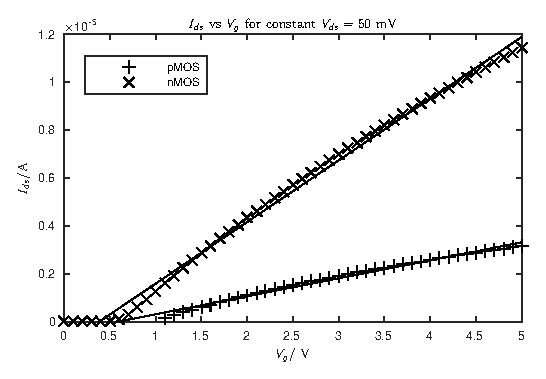
\includegraphics{ex1.eps}
    \caption{Experiment 1: \(I_{ds}\) as a function of \(V_g\) for \(V_{ds} = 50\) mV. The lines are fit to the points
        visibly above the x-axis. The fitted lines have equations \(I_{nMOS} = 2.576\cdot10^{-6}\frac{V_g}{\Omega}-9.872\cdot10^{-7} A\)
    and \(I_{pMOS} = 7.514\cdot10^{-7}\frac{V_g}{\Omega}-4.449\cdot10^{-7} A\).}
    \label{fig:ex1}
\end{figure}
Fig.~\ref{fig:ex1} shows \(I_{ds}\) as a function of \(V_g\) for nMOS and pMOS transistors with \(V_{ds} = 50\) mV.
For the pMOS transistor, current measurements for \(V_g < 1\) V are not shown because the K236 measured negative
values. This was because we placed the K236 between the supply rail and the drain terminal of the pMOS in order to
apply a small negative voltage. We also tried placing the K236 between ground and the drain terminal, in this case
we would measure very small positive currents below saturation as expected, however the currents measured above threshold
were far too small. Therefore we believe that the data displayed in this report is the most fitting.

From the fits we extract the \(\beta\) and \(V_T\) parameters according to the equation for current in the triode region
\begin{equation*}
    I_{ds} = \beta V_{ds} \left(V_g-V_T\right)
\end{equation*}

Finding

\begin{align*}
    \beta_{nMOS} &= 5.1521\cdot 10^{-5} \frac{1}{\Omega V} \quad V_{TnMOS} = 0.3832 V \\
    \beta_{pMOS} &= 1.5028\cdot 10^{-5} \frac{1}{\Omega V} \quad V_{TpMOS} = 0.5921 V
\end{align*}

It is obvious that the fits are not very accurate. There is systematic variation in the \(\beta\) parameter
caused by variation in the electron mobility \(\mu\). This must be the case as it is the only parameter in the
definition of \(\beta\) which can change, since
\begin{equation*}
    \beta = \mu C_{ox} \frac{W}{L}
\end{equation*}
Inspecting the graph, we find more fitting values of \(V_T\) to be
\begin{equation*}
    V_{TnMOS} = 0.65 V \quad V_{TpMOS} = 1.05 V
\end{equation*}
\begin{figure}
    \center
    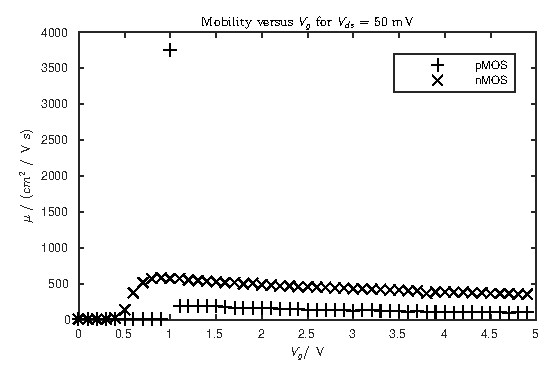
\includegraphics{extra.eps}
    \caption{Mobility as a function of \(V_g\) for \(V_ds = 50\) mV. For the pMOS transistor, the larger outlier indicates the
    gate voltage at which the measured current switched from negative to positive. We consider this to be a measurement artefact and it should
be ignored.}
    \label{fig:extra}
\end{figure}
\subsection{Mobility}
The carrier mobilities \(\mu_n\) and \(\mu_p\) of the nMOS and pMOS transistors can be seen in \reffig{fig:extra}. 
The mobility starts to decrease because the applied gate voltage results in an electric field orthogonal to the 
channel, which will pull the carriers towards the oxide where they will collide. Before the peak mobility level is reached,
applying a higher gate voltage results in a growth in the amount of carriers in the channel which increases mobility
more than the oxide collisions reduce it. The peak is reached when both effects are equal.

Ignoring the large outlier for the pMOS well-type transistor, we find the peak mobilities
\begin{equation*}
    \mu_{np} = 578.7 \frac{cm^2}{V s} \quad \mu_{pp} = 192.6 \frac{cm^2}{V s}
\end{equation*}
Resulting in a relative difference in peak mobility of
\begin{equation*}
    \frac{\mu_{np}}{\mu_{pp}} = 3.00
\end{equation*}
Which 20\% higher than the expected value of 2.5.

The peak mobilities are less than half of the bulk mobilities for electrons and holes. However, the bulk mobilities are 
given for majority carriers, and the peak mobilities we observe are for the carriers in the inversion layer which are 
minority carriers in the bulk, but majority carriers in the inversion layer.
\section{Experiment 2: Drain current in the saturation region}
\begin{figure}[!htb]
    \center
    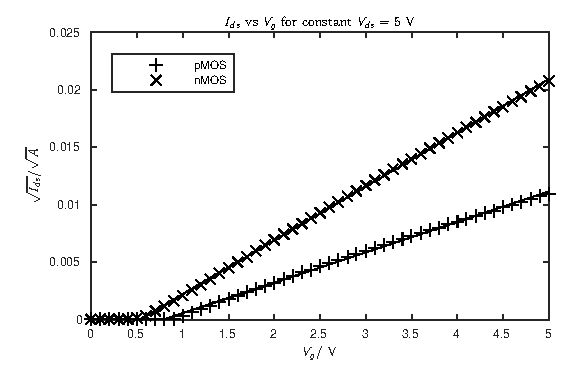
\includegraphics{ex2.eps}
    \caption{Experiment 2: \(\sqrt{I_{ds}}\) as a function of \(V_g\) for \(V_{ds} = 5\) V. Lines are fit to points visibly above the
        x-axis. The fitted lines have equations \(\sqrt{I_{pMOS}} = 2.648\cdot10^{-3} \frac{V_g}{\sqrt{\Omega V}} - 2.089\cdot10^{-3} \sqrt{A}\) and 
    \(\sqrt{I_{nMOS}} = 4.683\cdot10^{-3} \frac{V_g}{\sqrt{\Omega V}} - 2.469\cdot10^{-3}\sqrt{A}\).}
    \label{fig:ex2}
\end{figure}
The current through the transistors in saturation is shown in \reffig{fig:ex2}. From the linear fits we extrapolate
The \(\beta\) and \(V_T\) parameters according to the equation for current in saturation mode.

\begin{equation*}
    I_{ds} = \frac{\beta}{2}\left(V_g-V_T\right)
\end{equation*}

Finding

\begin{align*}
    \beta_{nMOS} &= 4.3861\cdot 10^{-5} \frac{1}{\Omega V} \quad V_{TnMOS} = 0.5272 V \\
    \beta_{pMOS} &= 1.4028\cdot 10^{-5} \frac{1}{\Omega V} \quad V_{TpMOS} = 0.7886 V
\end{align*}

The \(\beta\) values are similar to the ones obtained in the triode region, but the threshold values
are significantly different. Looking at the fitted lines, it is again immediately obvious that the 
extrapolated values for \(V_T\) are too low, just like in experiment 1.

We also tried fitting a quadratic function to the non-square root current. The quadratic fit is slightly better
in terms of mean error and residual error, however the difference is extremely small.

\section{Experiment 3: Drain characteristics of a single transistor at different saturation currents}
\begin{figure}[!htb]
    \center
    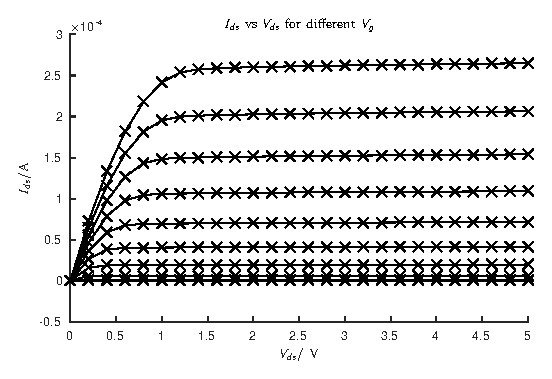
\includegraphics{ex3.eps}
    \caption{Experiment 3: \(I_{ds}\) versus \(V_{ds}\) in a 32/8 nMOS transistor, for 11 different values of \(V_g\) from 0.2 V to 2.2 V in steps of 0.2 V. 
    Lines are drawn between measurement points to help distinquish the curves from each other.}
    \label{fig:ex3}
\end{figure}
\begin{figure}[!htb]
    \center
    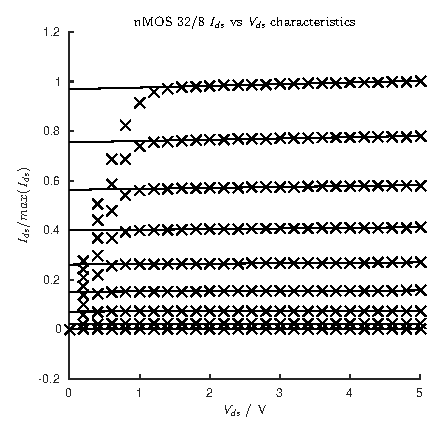
\includegraphics{ex3-2.eps}
    \caption{Experiment 3: The data shown in \reffig{fig:ex3}, but normalized and with lines fitted to points between \(V_{ds} = 1.8\) V and \(V_{ds} = 4\) V in order to find the Early voltage.
    The x-axis intercept is far behind the y-axis.}
    \label{fig:ex3-2}
\end{figure}
\begin{figure}[!htb]
    \center
    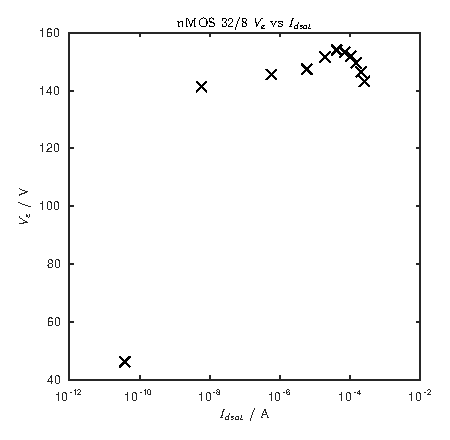
\includegraphics{ex3-3.eps}
    \caption{Experiment 3: The extrapolated Early voltage versus the extrapolated base saturation current.}
    \label{fig:ex3-3}
\end{figure}
Fig.~\ref{fig:ex3} shows the transistor current as a function of \(V_{ds}\) for several different values of \(V_g\). In Fig.~\ref{fig:ex3-2}, lines have been
fit to the saturation region of the currents. In Fig.~\ref{fig:ex3-3} the x-intercept of these lines is plotted against the y-intercept. These intercept
values are the Early voltage and \(I_{dsat}\) currents respectively. 

The Early voltage can be seen to not be constant. If we ignore the significant outlier, which is likely due to measurement error, the Early voltage increases
slightly with \(I_{dsat}\) and then drops rapidly. The value of the Early voltage is affected by the increase in saturation current when the gate voltage is increased,
as well as the increased slope of the current versus \(V_{ds}\) when there are more carriers in the channel for higher \(V_g\). If the slope of the 
current in saturation vs. \(V_{ds}\) grows faster than the increase in base saturation current, \(I_{dsat}\), then the Early voltage will drop, while it
will obviously rise if the opposite is true.

Therefore we can see from Fig.~\ref{fig:ex3-3} that the base saturation current increases faster than the slope while the Early voltage is going up, 
after which the Early voltage reaches a maximum and the base current begins to grow more slowly than the saturation current slope. This could be
caused by the interplay of channel length modulation by \(V_{ds}\) and \(V_g\). For lower gate voltages the pinchoff region will grow more quickly and
reduce the effective length of the channel, which increases current.

\end{document}
